\documentclass{beamer}
\beamertemplatenavigationsymbolsempty
\usecolortheme{beaver}
\usepackage{tikz}
\setbeamertemplate{blocks}[rounded=true, shadow=true]
\setbeamertemplate{footline}
[page number]
%
\usepackage{datetime}
\usepackage{hyperref}
\usepackage[utf8]{inputenc}
\usepackage[english,russian]{babel}
\usepackage{amssymb,amsfonts,amsmath,mathtext}
\usepackage{subfig}
\usepackage[all]{xy} % xy package for diagrams
\usepackage{array}
\usepackage{multicol} % many columns in slide
\usepackage{hyperref}
\usepackage{algpseudocode}
\hypersetup{
    colorlinks=true,
    linkcolor=blue,
    filecolor=magenta,      
    urlcolor=cyan,
    pdftitle={Overleaf Example},
    pdfpagemode=FullScreen,
    }

\usepackage{hhline} %tables
\usepackage{comment} %comments
\newcommand\marker[2]{{\fboxsep=0pt\colorbox{#1}{\strut #2}}}
\newcommand{\tvi}{f_i(x_i)}

\usepackage[style=ieee]{biblatex}
\addbibresource{biblio.bib}

% Your figures are here:
\graphicspath{ {../figures/} }
% latin bold lower
\newcommand{\ba}{\mathbf{a}} 
\newcommand{\bc}{\mathbf{c}} 
\newcommand{\be}{\mathbf{e}} 
\newcommand{\bh}{\mathbf{h}} 
\newcommand{\bp}{\mathbf{p}} 
\newcommand{\bt}{\mathbf{t}} 
\newcommand{\bs}{\mathbf{s}} 
\newcommand{\bu}{\mathbf{u}} 
\newcommand{\bv}{\mathbf{v}} 
\newcommand{\bw}{\mathbf{w}} 
\newcommand{\bx}{\mathbf{x}} 
\newcommand{\by}{\mathbf{y}} 
\newcommand{\bz}{\mathbf{z}} 
\newcommand{\bm}{\mathbf{m}} 

% latin bold upper
\newcommand{\bA}{\mathbf{A}} 
\newcommand{\bB}{\mathbf{B}} 
\newcommand{\bC}{\mathbf{C}} 
\newcommand{\bI}{\mathbf{I}} 
\newcommand{\bJ}{\mathbf{J}} 
\newcommand{\bL}{\mathbf{L}} 
\newcommand{\bM}{\mathbf{M}} 
\newcommand{\bP}{\mathbf{P}}
\newcommand{\bQ}{\mathbf{Q}} 
\newcommand{\bR}{\mathbf{R}} 
\newcommand{\bT}{\mathbf{T}} 
\newcommand{\bU}{\mathbf{U}} 
\newcommand{\bV}{\mathbf{V}} 
\newcommand{\bW}{\mathbf{W}} 
\newcommand{\bX}{\mathbf{X}} 
\newcommand{\bY}{\mathbf{Y}} 
\newcommand{\bZ}{\mathbf{Z}} 

% latin cal upper
\newcommand{\cF}{\mathcal{F}} 
\newcommand{\cG}{\mathcal{G}} 
\newcommand{\cI}{\mathcal{I}} 
\newcommand{\cL}{\mathcal{L}} 
\newcommand{\cM}{\mathcal{M}} 
\newcommand{\cN}{\mathcal{N}} 
\newcommand{\cS}{\mathcal{S}} 
\newcommand{\cT}{\mathcal{T}} 
\newcommand{\cW}{\mathcal{W}} 
\newcommand{\cX}{\mathcal{X}} 
\newcommand{\cZ}{\mathcal{Z}} 

% latin bb upper
\newcommand{\bbE}{\mathbb{E}} 
\newcommand{\bbI}{\mathbb{I}} 
\newcommand{\bbP}{\mathbb{P}} 
\newcommand{\bbR}{\mathbb{R}}
\newcommand{\bbX}{\mathbb{X}} 
\newcommand{\bbY}{\mathbb{Y}}
\newcommand{\bbW}{\mathbb{W}} 

% greek bold lower
\newcommand{\bepsilon}{\boldsymbol{\epsilon}} 
\newcommand{\btheta}{\boldsymbol{\theta}} 
\newcommand{\blambda}{\boldsymbol{\lambda}} 
\newcommand{\bpi}{\boldsymbol{\pi}} 
\newcommand{\bmu}{\boldsymbol{\mu}} 
\newcommand{\bsigma}{\boldsymbol{\sigma}} 
\newcommand{\bphi}{\boldsymbol{\phi}} 

% greek bold upper
\newcommand{\bSigma}{\boldsymbol{\Sigma}} 

\DeclareMathOperator*{\argmin}{arg\,min}
\DeclareMathOperator*{\argmax}{arg\,max}

% transpose
\newcommand{\T}{^{\text{\tiny\sffamily\upshape\mdseries T}}}

% my commands
\newcommand{\mbR}{{\mathbb R}}
\newcommand{\wt}[1]{\widetilde{#1}}
% \newcommand{\sto}{\gamma^*} % solition task 2 
% \newcommand{\stt}{\wt{\gamma}} % solition task 3
% \newcommand{\stf}{\overline{\gamma}} % solition task 4
% \newcommand{\tvi}{v_i}
\newcommand{\clip}{\texttt{clip}}
\include{metainfo}
\newcommand{\secref}[1]{\autoref{#1}. \nameref{#1}}
%----------------------------------------------------------------------------------------------------------

% \title[\hbox to 56mm]{\paperName}
% \author[И. М. Латыпов]{Latypov Ilgam Magdanovich}
% \institute[]{Moscow Institute of Physics and Technology, IAI MSU}


% \begin{document}
% \begin{frame}
%     \maketitle
%     \parbox{5,2cm}{NET conference 2024}
%     \hfill\parbox{3,4cm}{
%     \begin{small}        
%     \textbf{scientific supervisor:}\\
%         % \\к.т.н. Ю. В. Дорн
%         c.t.s. Dorn Y.V.
%     \end{small}
%     }
% \end{frame}
%----------------------------------------------------------------------------------------------------------

\title[\hbox to 56mm]{\paperName}
\author[И. М. Латыпов]{Latypov I. M., Dorn Y.V.}
\institute[]{Moscow Institute of Physics and Technology, IAI MSU}
\titlegraphic{NET conference 2024}

\begin{document}


% \begin{frame}
\begin{titlepage}
    % \maketitle
    \title[\hbox to 50mm]{\paperName}
    \author[И. М. Латыпов]{Latypov I. M., Dorn Y.V.}
    % \date{}
    % \today
    \institute[]{Moscow Institute of Physics and Technology, IAI MSU}
    \hfill
    \titlegraphic{NET conference 2024}
    % \today
\end{titlepage}
    
% \end{frame}
\begin{frame}{Пример для мотивации}
    При оптимизации топологии телекоммуникационных сетей необходимо балансировать между несколькими метриками:
    \begin{enumerate}
        \item Задержка в сети
        \item Пропускная способность
        \item Устойчивость сети
        \item ...
    \end{enumerate}
    Мы хотим получить сеть, которая будет хороша по всем метрикам, но для этого по каждой метрике требуется решить сложную задачу оптимизации.
\end{frame}
\begin{frame}{Проблема}
\begin{block}{Проблема}
    Существуют задачи многокритериальной оптимизации, в которых функции либо сложно вычислить, либо их перерасчёт невозможен.
\end{block}
\begin{block}{Исследовательская задача}
    Необходимо поставить задачу оптимизации для такого случая и предложить метод её приближенного решения. Метод должен работать только с уже известными значениями функций.
\end{block}
\begin{block}{Результаты}
\begin{list}{$\circ$}{}
    \item Поставлена и обобщена задача оптимизации для поиска конкурентного решения.
    \item Предложен метод нахождения приближенного решения для липшицевых и монотонных функций.
\end{list}
\end{block}
\end{frame}

\begin{frame}{Обозначения}
\begin{list}{$\circ$}{}
    \item $x \in \mbR^n$
    \item Множество решений $K$ является выпуклым, замкнутым и снабжено нормой $\|\cdot\|$
    \item функции $f_i: \mbR^n \rightarrow \mbR_+ ~~ i = \overline{1, m}$
    \item Пусть $x_i = \text{arg}\min_{x \in K} f_i(x)$. 
    \item $f_i(x_i) = \tvi$
\end{list}
\end{frame}

\begin{frame}{Задача оптимизации}

\begin{definition}[$\gamma$-конкурентная точка]
$x$ называется $\gamma$-конкурентной точкой, если для всех $i$ выполняется:
\begin{align}
    f_i(x) \leq (1 + \gamma) f_i^*
\end{align}
\end{definition}

\begin{block}{Задача оптимизации}
    \begin{align*}
    \min_{x, \gamma} \gamma & \tag{$T_1$}\label{opt:T1} \\    
    \text{s.t.}~~ & x \in K \\
                 &f_i(x) - \tvi \leq  \gamma \tvi, ~~  i\in\overline{1, m}
    \end{align*}
\end{block}
 
\end{frame}

\begin{frame}{Метод}
\begin{definition}[Условие Липшица]
\label{def:lipshitz_function}
    Функция $f : \mbR^n \rightarrow \mbR+$ удовлетворяет условию Липшица на $K$ с нормой $\|\cdot\|$:  
    $$
    \exists L > 0: ~ \forall x, y \in K:~  |f(x) - f(y) | \le L \|x -y\|
    $$
\end{definition}

\begin{itemize}
    \item Для всех $i = \overline{1, m}$ для $f_i(x):\mbR^n \rightarrow\mbR_+$:
        \begin{itemize}
            \item Удовлетворяет условию Липшица \ref{def:lipshitz_function} с константой $L_i$ на $K$.
            \item Вычислена в точке $x_i: \tvi$.
            \item Функция минимизируется.
        \end{itemize}
\end{itemize}
     Мы ищем $x \in K$, который является допустимым для \ref{opt:T1}. \\
     Метод не должен вычислять функции во время поиска решения.
\end{frame}

\begin{frame}{Метод}
\begin{block}{Предлагаемая переформулировка}      
    \begin{align*}
    \min_{x, \gamma} \gamma &  \tag{$T_2$}\label{opt:T2}  \\    
    \text{s.t.}~~ & x \in K \\
            & \| x - x_i\| \leq \frac{1}{L_i}(\gamma \tvi)  ~~ \forall i\in\overline{1,m}\\
                &\marker{gray}{$f_i(x) - \tvi \leq  \gamma \tvi ~~  i\in\overline{1, m}$ ~~~\text{(T1)}}
    \end{align*}
\end{block}

\begin{block}{Объяснение}
      Рассмотрим допустимые $x, \gamma$ из \ref{opt:T2}. Тогда для всех $i=\overline{1, m}$:
    \begin{equation}
        \|x_i - x\| \leq \frac{\gamma \tvi}{L_i}  \Rightarrow 
         |f_i(x) - \tvi| \leq \gamma \tvi
    \end{equation}
            \item Это означает, что $x, \gamma$ являются допустимыми для \ref{opt:T1}.
    \end{block}
\end{frame}

\begin{frame}{Пример для обобщения}

\begin{example}[Функция, которую нельзя пересчитать]\label{example:2}
    Служба доставки работала с различными стратегиями -- точками $x_i$ и вычисляла метрики -- $f_i(x_i)$. Теперь они хотят установить некоторые параметры, которые будут гарантировать значения метрик, если ситуация будет похожа на уже известные.
\end{example}

\begin{definition}[$\gamma$-конкурентная точка]
$x$ называется относительно $\gamma$-конкурентной точкой для функций $f_i$ и точек $x_i$, если для всех $i$:
\begin{align}
    f_i(x) \leq (1 + \gamma) f_i(x_i)
\end{align}
\end{definition}

\end{frame}

\begin{frame}{Метод}
    Мы можем использовать монотонность функций по параметрам для упрощения ограничений. Для этого введем оператор 
    $\clip_f: \mbR^n \times \mbR^n \rightarrow \mbR^n$:

\begin{equation}\label{def:clip}
    \clip_f(x, y)_i =         
    \begin{cases}
    \max(x_i - y_i, 0) & f ~\text{возрастает по} ~x_i \\
    \min(y_i - x_i, 0) & f ~\text{убывает по} ~ x_i \\
    x_i - y_i & \text{иначе}
        
    \end{cases}
\end{equation}

\baselineskip
\baselineskip

\begin{minipage}{0.3\textwidth}
\begin{align*}
\min c^Tx \\
Ax \leq b    
\end{align*}
\end{minipage}
\begin{minipage}{0.6\textwidth}
    
    \begin{figure}
 \resizebox{0.9\textwidth}{!}{



% Gradient Info
  
\tikzset {_fgowgr2lz/.code = {\pgfsetadditionalshadetransform{ \pgftransformshift{\pgfpoint{0 bp } { 0 bp }  }  \pgftransformrotate{0 }  \pgftransformscale{2 }  }}}
\pgfdeclarehorizontalshading{_9dhn7icul}{150bp}{rgb(0bp)=(0.88,0.81,0.81);
rgb(57.410714285714285bp)=(0.88,0.81,0.81);
rgb(61.69642857142857bp)=(1,1,1);
rgb(100bp)=(1,1,1)}

% Gradient Info
  
\tikzset {_9i12ftknc/.code = {\pgfsetadditionalshadetransform{ \pgftransformshift{\pgfpoint{0 bp } { 0 bp }  }  \pgftransformrotate{0 }  \pgftransformscale{2 }  }}}
\pgfdeclarehorizontalshading{_8naggw73p}{150bp}{rgb(0bp)=(0.82,0.65,0.65);
rgb(56.160714285714285bp)=(0.82,0.65,0.65);
rgb(62.5bp)=(1,1,1);
rgb(100bp)=(1,1,1)}
\tikzset{every picture/.style={line width=0.75pt}} %set default line width to 0.75pt        

\begin{tikzpicture}[x=0.75pt,y=0.75pt,yscale=-1,xscale=1]
%uncomment if require: \path (0,299); %set diagram left start at 0, and has height of 299

%Rounded Single Corner Rect [id:dp17495013363449963] 
\draw  [draw opacity=0][shading=_9dhn7icul,_fgowgr2lz] (195,133.87) .. controls (195,110.75) and (213.75,92) .. (236.87,92) -- (476,92) -- (476,271) -- (195,271) -- cycle ;
%Shape: Rectangle [id:dp7232887315160181] 
\draw  [draw opacity=0][shading=_8naggw73p,_9i12ftknc] (244,137) -- (476,137) -- (476,271) -- (244,271) -- cycle ;
%Shape: Axis 2D [id:dp342306719128316] 
\draw [line width=1.5]  (88,271) -- (475,271)(126.7,55) -- (126.7,295) (468,266) -- (475,271) -- (468,276) (121.7,62) -- (126.7,55) -- (131.7,62)  ;
%Straight Lines [id:da012330496298091465] 
\draw    (244,137) -- (244,271) ;
%Straight Lines [id:da39899782764903446] 
\draw    (244,137) -- (476,137) ;
%Flowchart: Connector [id:dp12740503153870053] 
\draw  [fill={rgb, 255:red, 0; green, 0; blue, 0 }  ,fill opacity=1 ] (242.5,137) .. controls (242.5,136.17) and (243.17,135.5) .. (244,135.5) .. controls (244.83,135.5) and (245.5,136.17) .. (245.5,137) .. controls (245.5,137.83) and (244.83,138.5) .. (244,138.5) .. controls (243.17,138.5) and (242.5,137.83) .. (242.5,137) -- cycle ;
%Flowchart: Connector [id:dp006258619069160698] 
\draw  [fill={rgb, 255:red, 0; green, 0; blue, 0 }  ,fill opacity=1 ] (358.5,75.87) .. controls (358.5,75.04) and (359.17,74.37) .. (360,74.37) .. controls (360.83,74.37) and (361.5,75.04) .. (361.5,75.87) .. controls (361.5,76.7) and (360.83,77.37) .. (360,77.37) .. controls (359.17,77.37) and (358.5,76.7) .. (358.5,75.87) -- cycle ;
%Flowchart: Connector [id:dp8712626682658107] 
\draw  [fill={rgb, 255:red, 0; green, 0; blue, 0 }  ,fill opacity=1 ] (360.5,136.5) .. controls (360.5,136.22) and (360.28,136) .. (360,136) .. controls (359.72,136) and (359.5,136.22) .. (359.5,136.5) .. controls (359.5,136.78) and (359.72,137) .. (360,137) .. controls (360.28,137) and (360.5,136.78) .. (360.5,136.5) -- cycle ;
%Straight Lines [id:da7671828037724451] 
\draw    (360,137) -- (360,76.37) ;
\draw [shift={(360,74.37)}, rotate = 90] [color={rgb, 255:red, 0; green, 0; blue, 0 }  ][line width=0.75]    (10.93,-3.29) .. controls (6.95,-1.4) and (3.31,-0.3) .. (0,0) .. controls (3.31,0.3) and (6.95,1.4) .. (10.93,3.29)   ;
%Straight Lines [id:da24275942902753656] 
\draw    (244,213) -- (161,213) ;
\draw [shift={(159,213)}, rotate = 360] [color={rgb, 255:red, 0; green, 0; blue, 0 }  ][line width=0.75]    (10.93,-3.29) .. controls (6.95,-1.4) and (3.31,-0.3) .. (0,0) .. controls (3.31,0.3) and (6.95,1.4) .. (10.93,3.29)   ;
%Flowchart: Connector [id:dp2595803353635131] 
\draw  [fill={rgb, 255:red, 0; green, 0; blue, 0 }  ,fill opacity=1 ] (544.5,50.5) .. controls (544.5,50.22) and (544.28,50) .. (544,50) .. controls (543.72,50) and (543.5,50.22) .. (543.5,50.5) .. controls (543.5,50.78) and (543.72,51) .. (544,51) .. controls (544.28,51) and (544.5,50.78) .. (544.5,50.5) -- cycle ;
%Flowchart: Connector [id:dp33830242400783717] 
\draw  [fill={rgb, 255:red, 0; green, 0; blue, 0 }  ,fill opacity=1 ] (244,213) .. controls (244,212.72) and (243.78,212.5) .. (243.5,212.5) .. controls (243.22,212.5) and (243,212.72) .. (243,213) .. controls (243,213.28) and (243.22,213.5) .. (243.5,213.5) .. controls (243.78,213.5) and (244,213.28) .. (244,213) -- cycle ;
%Flowchart: Connector [id:dp03082330545193468] 
\draw  [fill={rgb, 255:red, 0; green, 0; blue, 0 }  ,fill opacity=1 ] (157.5,213) .. controls (157.5,212.17) and (158.17,211.5) .. (159,211.5) .. controls (159.83,211.5) and (160.5,212.17) .. (160.5,213) .. controls (160.5,213.83) and (159.83,214.5) .. (159,214.5) .. controls (158.17,214.5) and (157.5,213.83) .. (157.5,213) -- cycle ;
%Straight Lines [id:da45681418240068217] 
\draw    (244,137) -- (209.08,82.68) ;
\draw [shift={(208,81)}, rotate = 57.26] [color={rgb, 255:red, 0; green, 0; blue, 0 }  ][line width=0.75]    (10.93,-3.29) .. controls (6.95,-1.4) and (3.31,-0.3) .. (0,0) .. controls (3.31,0.3) and (6.95,1.4) .. (10.93,3.29)   ;
%Flowchart: Connector [id:dp6452215731100408] 
\draw  [fill={rgb, 255:red, 0; green, 0; blue, 0 }  ,fill opacity=1 ] (206.5,81) .. controls (206.5,80.17) and (207.17,79.5) .. (208,79.5) .. controls (208.83,79.5) and (209.5,80.17) .. (209.5,81) .. controls (209.5,81.83) and (208.83,82.5) .. (208,82.5) .. controls (207.17,82.5) and (206.5,81.83) .. (206.5,81) -- cycle ;
%Straight Lines [id:da32694358794837974] 
\draw  [dash pattern={on 0.84pt off 2.51pt}]  (289.52,136.5) -- (289.98,91) ;
\draw [shift={(289.98,91)}, rotate = 270.58] [color={rgb, 255:red, 0; green, 0; blue, 0 }  ][line width=0.75]    (10.93,-4.9) .. controls (6.95,-2.3) and (3.31,-0.67) .. (0,0) .. controls (3.31,0.67) and (6.95,2.3) .. (10.93,4.9)   ;
\draw [shift={(289.52,136.5)}, rotate = 90.58] [color={rgb, 255:red, 0; green, 0; blue, 0 }  ][line width=0.75]    (10.93,-4.9) .. controls (6.95,-2.3) and (3.31,-0.67) .. (0,0) .. controls (3.31,0.67) and (6.95,2.3) .. (10.93,4.9)   ;

% Text Node
\draw (456,233) node [anchor=north west][inner sep=0.75pt]  [font=\LARGE] [align=left] {$\displaystyle 1$};
% Text Node
\draw (137,43) node [anchor=north west][inner sep=0.75pt]  [font=\LARGE] [align=left] {$\displaystyle 2$};
% Text Node
\draw (246,95.5) node [anchor=north west][inner sep=0.75pt]  [font=\huge] [align=left] {$\displaystyle y$};
% Text Node
\draw (353,37) node [anchor=north west][inner sep=0.75pt]  [font=\huge] [align=left] {$\displaystyle x_{1}$};
% Text Node
\draw (151,172) node [anchor=north west][inner sep=0.75pt]  [font=\huge] [align=left] {$\displaystyle x_{3}$};
% Text Node
\draw (201,43) node [anchor=north west][inner sep=0.75pt]  [font=\huge] [align=left] {$\displaystyle x$};
% Text Node
\draw (351,142) node [anchor=north west][inner sep=0.75pt]  [font=\huge] [align=left] {$\displaystyle y_{1}$};
% Text Node
\draw (255,194) node [anchor=north west][inner sep=0.75pt]  [font=\huge] [align=left] {$\displaystyle y_{3}$};
% Text Node
\draw (294,101) node [anchor=north west][inner sep=0.75pt]  [font=\LARGE] [align=left] {$\displaystyle r$};


\end{tikzpicture}

    } 
\end{figure}

\end{minipage}

\end{frame}

\begin{frame}{Метод}
    \begin{align*}
        \min_{x, \gamma} \gamma & \tag{$T_2$}\label{opt:T2} \\
        \text{s.t. } &x \in K \\
                     &\| x - x_i\| \leq \frac{1}{L_i}(\gamma \tvi)  ~~ \forall i\in\overline{1,m}
    \end{align*}
    $\longmapsto$
    \begin{align*}
    \min_{x, \gamma} \gamma & \tag{$T_3$}\label{opt:T3} \\
    \text{s.t. } &x \in K \\
                 &\|clip(x,x_i, f_i)\| \leq \frac{1}{L_i}(\gamma \tvi) ~~ \forall i\in\overline{1,m}
    \end{align*}
\end{frame}

\begin{frame}{Теоретические результаты}
\newtheorem{theorem}{Теорема}
    \begin{align*}
    \min_{x, \gamma} \gamma & \tag{$T_3$}\label{opt:T3} \\
    \text{s.t. } &x \in K \\
                 &\|clip_{f_i}(x,x_i)\| \leq \frac{1}{L_i}(\gamma f_i(x_i)) ~~ \forall i\in\overline{1,m} \\
                &\marker{gray}{$f_i(x) - \tvi \leq  \gamma \tvi ~~  i\in\overline{1, m}$ ~~~\text{(T1)}}
    \end{align*}
    
\begin{theorem}[Latypov, 2024]
    Решение $(x, \gamma)$ задачи \ref{opt:T3} является выполнимой точкой для  \ref{opt:T1}
\end{theorem}

\newcommand{\sto}{\gamma^*} % solition task 2 
\newcommand{\stt}{\wt{\gamma}} % solition task 3
\newcommand{\stf}{\overline{\gamma}} % solition task 4
\newcommand{\km}{\kappa{\max}}
\begin{theorem}[Latypov, 2024]
Пусть $\sto$ является решением задачи \ref{opt:T3}. Если у нас есть аппроксимации констант Липшица $\widetilde{L_i} = \kappa_i L_i$, тогда решая задачу \ref{opt:T3}, в которой константы Липшица заменены на $\widetilde{L_i}$, мы получаем $x$, для которого $|f(x) - \tvi| \leq \frac{\kappa_{\max}}{\kappa_i} \sto \tvi$. Здесь $\kappa_{\max} = \max_{i = \overline{1,m}} \kappa_i$.
\end{theorem}
\end{frame}
\begin{frame}{Эксперимент: Введение}
\begin{block}{Функция}
    \begin{align*}
        f(b, \xi) = c_b^T \cdot b + c_a^T \cdot \max(r_{\xi} - b, 0)
    \end{align*}
    Каждый вектор из $\mbR^n$, $c_b \le c_a$ покомпонентно.
\end{block}

\begin{block}{Пояснение}
    Представим, что компания потребляет случайное количество ресурсов $r_{\xi}$ в каждом периоде. 
В начале периода можно купить $b$ по более низкой цене. 
При необходимости они докупают недостающие ресурсы по более высокой цене.
\end{block}
    \begin{itemize}
        \item Компания проработала $m$ периодов и наблюдала для $i \in \overline{1, m}: r_\xi, c_b^i, c_a^i$ количество ресурсов $b_i$. 
        \item $K = \{b: c_b^T \cdot b \leq B \}$
    \end{itemize}
\end{frame}

\begin{frame}{Эксперимент: результаты}

    \begin{figure}
    \centering
    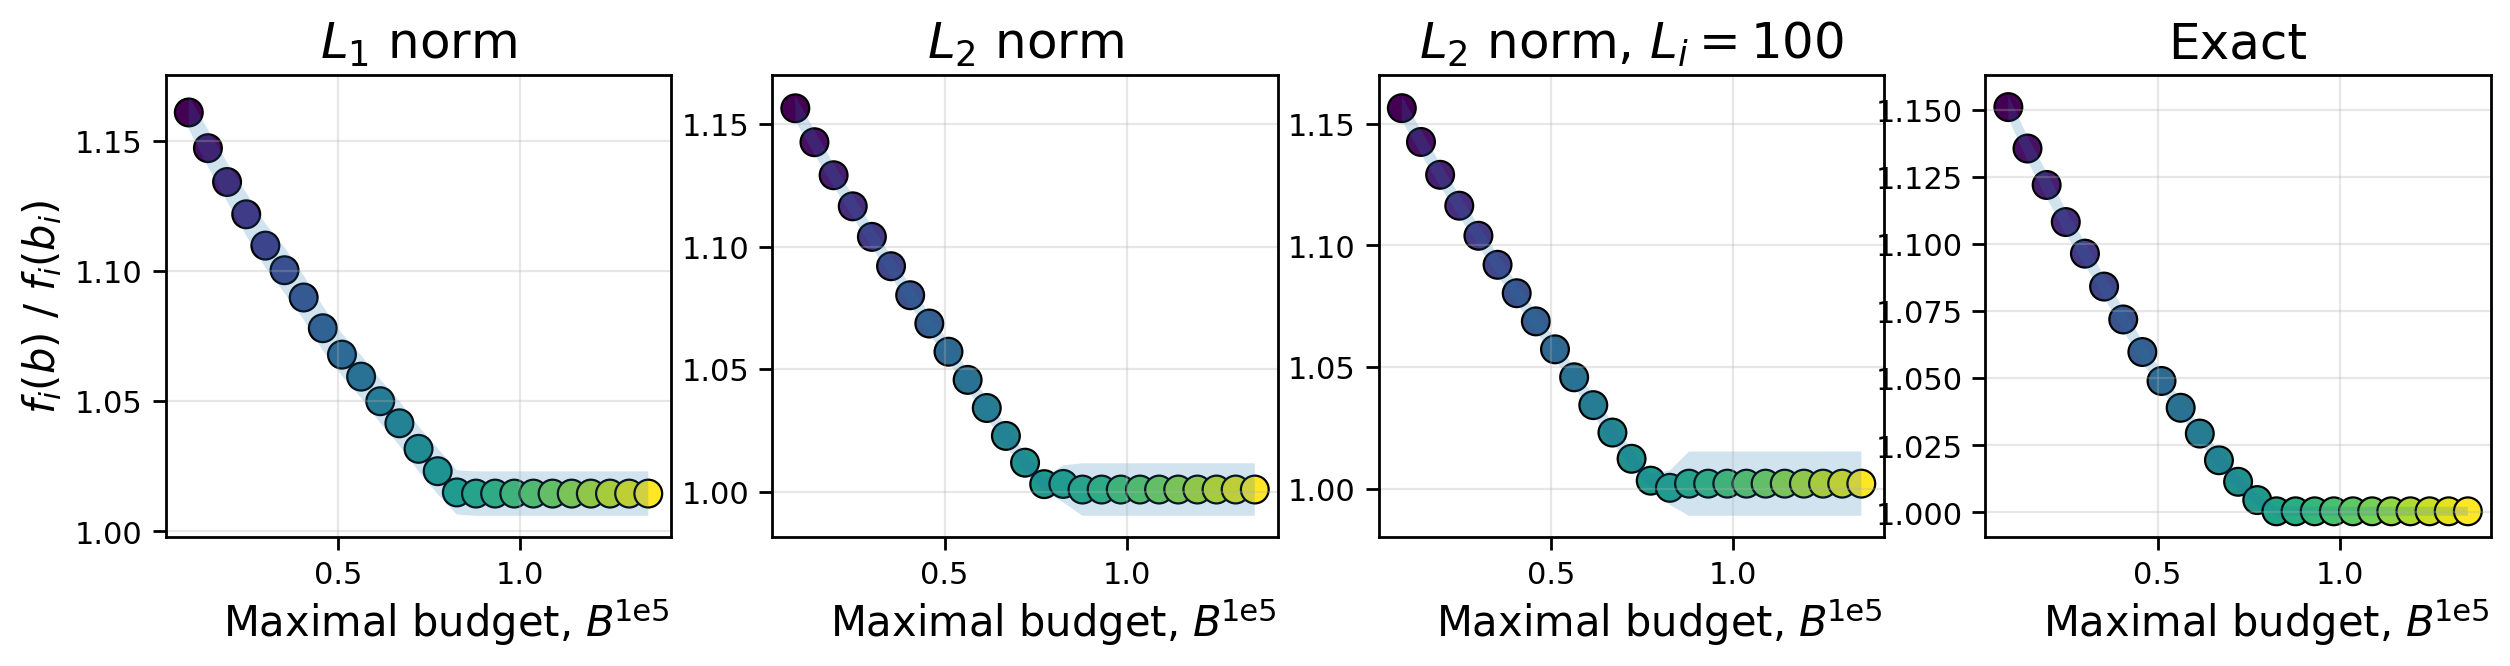
\includegraphics[width=\textwidth]{figures/simplest/relations.png}
                \caption{Зависимость относительных приростов функции от бюджета для разных подходов.}
        \label{fig:enter-label}
    \end{figure}
    
\end{frame}

\begin{frame}{Эксперимент: результаты}
    \begin{figure}
        \centering
        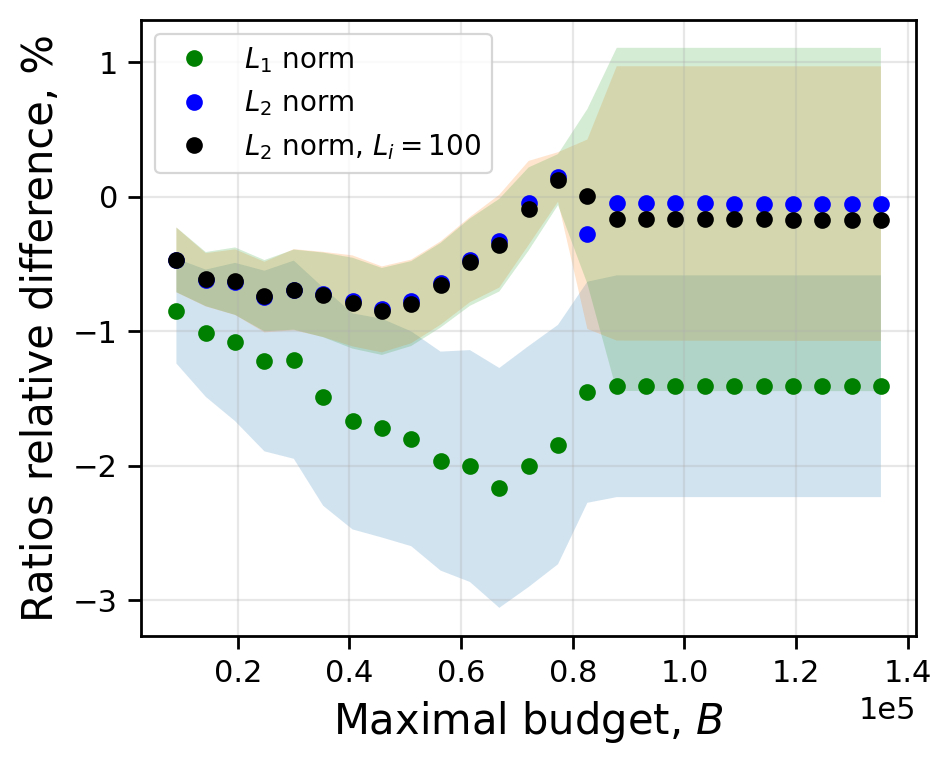
\includegraphics[width=0.5\textwidth]{figures/simplest/relative_difference.png}
        \caption{Относительная разница результатов аппроксимаций с точным решением.}
        \label{fig:enter-label}
    \end{figure}
    
\end{frame}

\begin{frame}{Итоги}
    Выносится на защиту:
    \begin{itemize}
        \item Предложен метод скаляризации с хорошей интерпретацией и метод поиска приближенного решения, не требующий вычисления функций.
        \item Проведен теоретический анализ для случая неточных параметров.
        \item Представленные эксперименты демонстрируют полезность предложенного метода.
    \end{itemize}
\end{frame}


\end{document}


    